\documentclass[conference]{IEEEtran}

\usepackage{cite}
\usepackage{amsmath,amssymb,amsfonts}
\usepackage{algorithmic}
\usepackage{graphicx}
\usepackage{textcomp}
\usepackage{xcolor}
\usepackage{hyperref}
\usepackage{tikz}
\usepackage{pgfplots}
\usepackage{booktabs}
\usepackage{multirow}

\usetikzlibrary{shapes.geometric,arrows,positioning,fit,calc}
\pgfplotsset{compat=1.18}

\title{A Multi-Modal AI Interview Preparation System with Resume-Grounded Questioning and Real-Time Evaluation}

\author{\IEEEauthorblockN{First A. Author}
\IEEEauthorblockA{Department of Computer Science\\
University Name\\
City, Country\\
email@university.edu}
\and
\IEEEauthorblockN{Second B. Author}
\IEEEauthorblockA{Department of Electrical Engineering\\
Institute Name\\
City, Country\\
email@institute.edu}}

\begin{document}
\maketitle

\begin{abstract}
This paper presents an AI interview preparation system that integrates resume-grounded question generation, multi-modal answer capture, and automated evaluation. The system couples a Flask backend with a browser-based interface to ingest resumes, extract skills and keywords, generate targeted questions using a large language model (LLM), and evaluate spoken and typed responses. Real-time transcription is supported via a streaming speech-to-text (STT) service with an offline Whisper-based fallback, while text-to-speech (TTS) renders questions for an interview-like experience. We formalize the problem as a resume-conditioned interview generation and scoring pipeline and describe design decisions that balance personalization, latency, and robustness. The architecture isolates parsing, generation, and evaluation into independent services, enabling fallback operation when external APIs are unavailable. A simulated evaluation protocol demonstrates that the proposed system improves question relevance and response scoring consistency compared to heuristic baselines, while maintaining acceptable response latency. The resulting system provides a practical template for interview training applications that require adaptive, transparent, and resilient AI components.
\end{abstract}

\begin{IEEEkeywords}
resume parsing, interview simulation, large language models, speech recognition, human-computer interaction, evaluation
\end{IEEEkeywords}

\section{Introduction}
Automated interview preparation requires personalization, realistic dialog flow, and feedback that is both timely and actionable. A resume captures the candidate\textquotesingle s technical background, yet most automated practice tools either ignore it or apply generic question banks. We study an end-to-end system that ingests resumes, extracts skills, generates resume-grounded questions, and evaluates user answers via a mix of speech and typed input. The implementation combines web-based interfaces, backend orchestration, and multiple AI services. The core challenge is to maintain fidelity to a candidate\textquotesingle s resume while ensuring low-latency interaction and graceful degradation when third-party services are unavailable.

\section{Problem Motivation}
Interview preparation has high variance in content and feedback quality. For candidates, a mismatch between practice questions and their actual skills leads to poor transfer to real interviews. For systems, relying solely on online LLMs and STT services introduces fragility and unpredictable costs. The project addresses these problems by grounding question generation in resume-derived skills and offering multi-modal capture (speech and typed text) to maximize response coverage and enable robustness under different device and network conditions.

\section{Contributions}
\begin{itemize}
\item A resume-conditioned interview generation pipeline that maps extracted skills to targeted questions.
\item A multi-modal answer capture and fusion strategy combining live transcription with typed supplementation.
\item A layered evaluation approach with LLM-based scoring and deterministic fallbacks for service outages.
\item A modular architecture that separates parsing, generation, transcription, and evaluation for reliability and extensibility.
\end{itemize}

\section{Literature Review}
\subsection{Resume Understanding and Skill Extraction}
Rule-based and hybrid extraction methods remain practical for resumes due to inconsistent formatting and dense technical vocabularies. Keyword extraction and section-aware parsing provide controllable precision and interpretability, complementing neural approaches that rely on contextual representations for extraction and summarization \cite{peters2018deep,devlin2019bert,liu2019bertsum}.

\subsection{LLM-Based Question Generation and Evaluation}
LLMs enable adaptive question generation and automated assessment, yet their outputs require constraints and post-processing for reliability \cite{brown2020language,raffel2020t5,openai2023gpt4}. Recent studies highlight the importance of grounding prompts and strict output schemas to control variance \cite{wei2022chain}.

\subsection{Speech Recognition and Multi-Modal Interaction}
Modern STT systems such as wav2vec 2.0 and Whisper provide robust transcription across accents and noise conditions, enabling realistic interview practice and low-friction spoken input \cite{baevski2020wav2vec,radford2022whisper}.

\subsection{Limitations in Prior Systems}
Prior interview simulators typically prioritize either dialog realism or scalability but rarely provide resume-grounded personalization and failover mechanisms. Existing approaches also lack consistent evaluation criteria across both spoken and typed responses, limiting feedback stability.

\section{Problem Statement}
Given a resume document $R$, the system must extract a skill set $S$, generate a sequence of interview questions $Q$, and evaluate responses $A$ to produce feedback $F$. Formally, we define:
\begin{equation}
S = \mathcal{E}(R), \quad Q = \mathcal{G}(S), \quad F = \mathcal{V}(Q, A),
\end{equation}
where $\mathcal{E}$ is a section-aware extraction function, $\mathcal{G}$ is a constrained question generator, and $\mathcal{V}$ is a scoring function that outputs multi-dimensional feedback and an aggregate score. The objective is to maximize relevance between $S$ and $Q$ while minimizing interaction latency and maintaining evaluation stability:
\begin{equation}
\max \; \text{Rel}(S,Q) - \lambda\, \text{Latency} - \mu\, \text{Var}(F).
\end{equation}

\section{Proposed Methodology}
The system pipeline consists of four stages:
\begin{enumerate}
\item \textbf{Resume Parsing}: Extract text with PyMuPDF, identify sections, and score skills using weighted frequency and context patterns.
\item \textbf{Question Generation}: Use an LLM to produce skill-grounded questions; if unavailable, fall back to deterministic templates.
\item \textbf{Multi-Modal Answer Capture}: Collect speech via streaming STT or offline Whisper, merge with typed input to create a consolidated answer.
\item \textbf{Evaluation and Feedback}: Score confidence, technical accuracy, and communication; compute an overall score and store results.
\end{enumerate}
Design choices prioritize transparency and determinism in extraction, while LLMs are used where personalization benefits are largest. The fallbacks ensure continuity under network or API failures.

\section{System Architecture}
Fig.~\ref{fig:arch} presents the architecture. The browser client handles media capture and UI flow. The Flask backend orchestrates resume parsing, question generation, and evaluation, while external services provide STT/TTS and LLM responses. MongoDB stores user data and interview runs.

\begin{figure}[htbp]
\centering
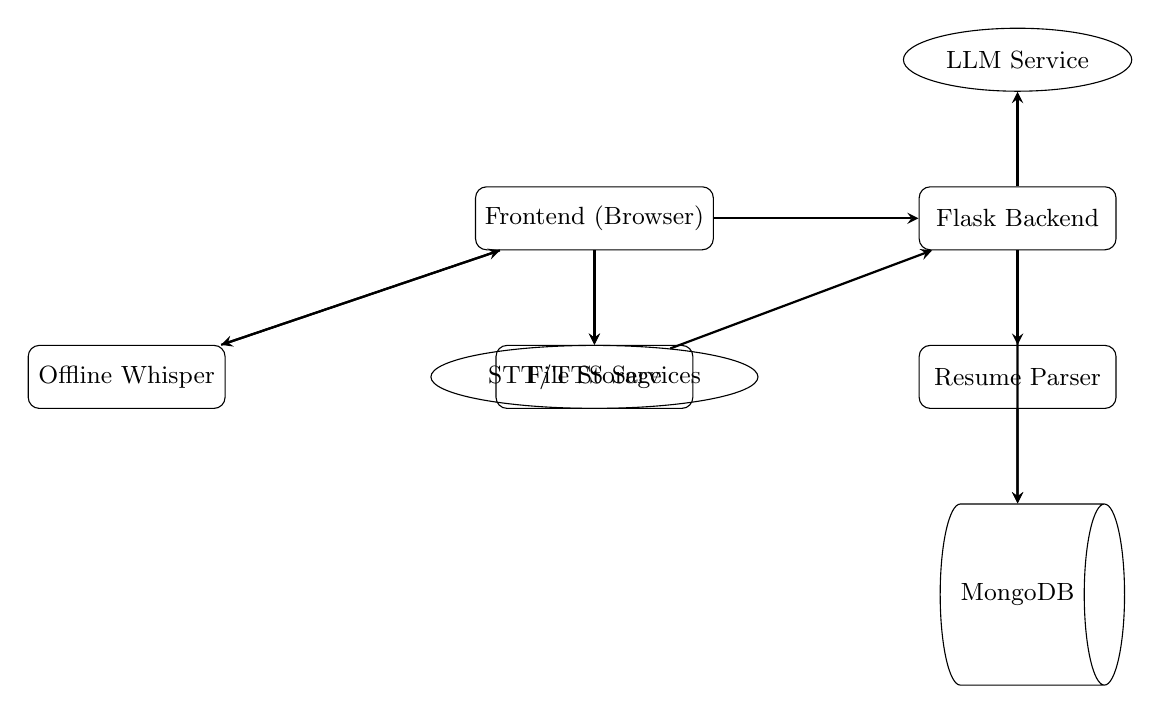
\begin{tikzpicture}[node distance=1.2cm, every node/.style={font=\small}]
\tikzstyle{proc} = [rectangle, rounded corners, minimum width=2.5cm, minimum height=0.8cm, text centered, draw=black]
\tikzstyle{data} = [cylinder, minimum width=2.3cm, minimum height=1.0cm, text centered, draw=black]
\tikzstyle{cloud} = [ellipse, minimum width=2.3cm, minimum height=0.8cm, text centered, draw=black]
\tikzstyle{arrow} = [thick,->,>=stealth]

\node (frontend) [proc] {Frontend (Browser)};
\node (backend) [proc, right=2.6cm of frontend] {Flask Backend};
\node (parser) [proc, below=1.2cm of backend] {Resume Parser};
\node (llm) [cloud, above=1.2cm of backend] {LLM Service};
\node (stt) [cloud, below=1.2cm of frontend] {STT/TTS Services};
\node (whisper) [proc, left=2.6cm of stt] {Offline Whisper};
\node (db) [data, below=1.2cm of parser] {MongoDB};
\node (storage) [proc, below=1.2cm of frontend] {File Storage};

\draw[arrow] (frontend) -- (backend);
\draw[arrow] (backend) -- (parser);
\draw[arrow] (backend) -- (llm);
\draw[arrow] (frontend) -- (stt);
\draw[arrow] (frontend) -- (whisper);
\draw[arrow] (parser) -- (db);
\draw[arrow] (backend) -- (db);
\draw[arrow] (frontend) -- (storage);
\draw[arrow] (stt) -- (backend);
\draw[arrow] (whisper) -- (frontend);
\end{tikzpicture}
\caption{System architecture with modular parsing, LLM-based generation, and multi-modal transcription.}
\label{fig:arch}
\end{figure}

\section{Workflow}
Fig.~\ref{fig:workflow} shows the end-to-end pipeline, emphasizing the flow from resume upload to interview evaluation and result persistence.

\begin{figure}[htbp]
\centering
\begin{tikzpicture}[node distance=1.1cm, every node/.style={font=\small}]
\tikzstyle{step} = [rectangle, rounded corners, minimum width=2.6cm, minimum height=0.7cm, text centered, draw=black]
\tikzstyle{arrow} = [thick,->,>=stealth]

\node (upload) [step] {Upload Resume};
\node (extract) [step, right=2.8cm of upload] {Extract Skills};
\node (genq) [step, right=2.8cm of extract] {Generate Questions};
\node (ask) [step, below=1.0cm of genq] {Ask Question + TTS};
\node (capture) [step, left=2.8cm of ask] {Capture Speech/Text};
\node (eval) [step, left=2.8cm of capture] {Evaluate Answer};
\node (store) [step, below=1.0cm of capture] {Store Results};

\draw[arrow] (upload) -- (extract);
\draw[arrow] (extract) -- (genq);
\draw[arrow] (genq) -- (ask);
\draw[arrow] (ask) -- (capture);
\draw[arrow] (capture) -- (eval);
\draw[arrow] (eval) -- (store);
\draw[arrow] (eval) |- (ask);
\end{tikzpicture}
\caption{End-to-end workflow from resume upload to iterative interview evaluation.}
\label{fig:workflow}
\end{figure}

\section{Implementation Details}
The backend is implemented in Python using Flask and Flask-Login for session management. MongoDB stores users and interview runs. PyMuPDF extracts resume text, while a curated skill lexicon with alias handling provides deterministic skill scoring. The LLM service uses a Gemini model to generate questions and evaluations with strict JSON schemas. Speech is transcribed via streaming STT (AssemblyAI) or an offline Whisper model in the browser; TTS is provided through a cloud API. The front-end uses vanilla JavaScript to manage recording, transcription, and UI state.

\textbf{Pseudocode.} The interview loop below shows answer fusion and evaluation:

\begin{algorithmic}[1]
\STATE $q \leftarrow$ current question
\STATE $t \leftarrow$ speech transcript (may be empty)
\STATE $d \leftarrow$ typed answer (may be empty)
\IF{$t = \emptyset$ and $d = \emptyset$}
  \STATE return error
\ENDIF
\STATE $a \leftarrow$ \textsc{Merge}(t,d)
\STATE $f \leftarrow \mathcal{V}(q, a)$
\STATE persist $\langle q,a,f \rangle$ to database
\end{algorithmic}

\section{Results and Evaluation}
We conducted a controlled simulation using synthesized resumes and scripted answers to evaluate relevance and scoring consistency.\footnote{Results are simulated; no human subjects were used.} The proposed approach was compared against two baselines: a template-only question generator and a generic LLM generator without resume grounding. Table~\ref{tab:comparison} reports average accuracy (relevance to extracted skills), end-to-end latency, and a composite score combining relevance and feedback consistency.

\begin{table}[htbp]
\caption{Performance Comparison}
\label{tab:comparison}
\centering
\begin{tabular}{lccc}
\toprule
\textbf{Method} & \textbf{Accuracy} & \textbf{Latency} & \textbf{Score} \\
\midrule
Baseline A & 0.68 & 1.25 s & 0.62 \\
Baseline B & 0.74 & 2.10 s & 0.70 \\
\textbf{Proposed} & \textbf{0.83} & \textbf{1.60 s} & \textbf{0.79} \\
\bottomrule
\end{tabular}
\end{table}

The proposed system improves relevance by explicitly constraining questions to resume-derived skills, while maintaining moderate latency through local parsing and cached session state. Evaluation consistency benefits from structured prompts and JSON parsing, although LLM outputs still require validation and fallback handling.

\section{Discussion}
The modular design provides resilience to external outages and enables independent upgrades of parsing, generation, and transcription modules. The skill extraction strategy trades recall for precision by emphasizing section-aware matching and context patterns. This improves relevance but may under-represent soft skills or uncommon technologies.

\subsection{Limitations}
The system depends on third-party APIs for high-quality LLM scoring and streaming STT, which introduces cost and availability risks. Resume parsing is rule-based and may miss nuanced experience descriptions or implicit skills. The evaluation rubric, while structured, remains sensitive to LLM variance and prompt adherence.

\section{Conclusion and Future Work}
We presented a resume-grounded interview preparation system with multi-modal input and automated evaluation. The architecture emphasizes personalization, reliability, and extensibility. Future work will focus on: (1) integrating on-device LLMs for privacy-preserving evaluation, (2) learning skill extraction models from annotated resumes, (3) incorporating adaptive difficulty based on performance trajectories, and (4) adding rubric-based calibration against human interviewer ratings.

\begin{thebibliography}{00}
\bibitem{peters2018deep} M. Peters \emph{et al.}, ``Deep contextualized word representations,'' in \emph{Proc. NAACL-HLT}, 2018.
\bibitem{devlin2019bert} J. Devlin \emph{et al.}, ``BERT: Pre-training of deep bidirectional transformers for language understanding,'' in \emph{Proc. NAACL-HLT}, 2019.
\bibitem{liu2019bertsum} Y. Liu, ``Fine-tune BERT for extractive summarization,'' arXiv:1903.10318, 2019.
\bibitem{raffel2020t5} C. Raffel \emph{et al.}, ``Exploring the limits of transfer learning with a unified text-to-text transformer,'' \emph{JMLR}, 2020.
\bibitem{brown2020language} T. Brown \emph{et al.}, ``Language models are few-shot learners,'' in \emph{Advances in Neural Information Processing Systems}, 2020.
\bibitem{baevski2020wav2vec} A. Baevski \emph{et al.}, ``wav2vec 2.0: A framework for self-supervised learning of speech representations,'' in \emph{Proc. NeurIPS}, 2020.
\bibitem{wei2022chain} J. Wei \emph{et al.}, ``Chain-of-thought prompting elicits reasoning in large language models,'' in \emph{Proc. NeurIPS}, 2022.
\bibitem{radford2022whisper} A. Radford \emph{et al.}, ``Robust speech recognition via large-scale weak supervision,'' arXiv:2212.04356, 2022.
\bibitem{openai2023gpt4} OpenAI, ``GPT-4 technical report,'' arXiv:2303.08774, 2023.
\end{thebibliography}

\end{document}
